% VUT FIT MITAI
% MSZ 2021/2022
% Author: Vladimir Dusek
% Login: xdusek27

%%%%%%%%%%%%%%%%%%%%%%%%%%%%%%%%%%%%%%%%%%%%%%%%%%%%%%%%%%%%%%%%%%%%%%%%%%%%%%%%

% Path to figures
\graphicspath{{sui/klasifikace_generativni_diskriminativni/figures}}

%%%%%%%%%%%%%%%%%%%%%%%%%%%%%%%%%%%%%%%%%%%%%%%%%%%%%%%%%%%%%%%%%%%%%%%%%%%%%%%%

\chapter{SUI~--~Generativní modely a diskriminativní přístup ke klasifikaci (gaussovský klasifikátor, logistická regrese, ...)}

%%%%%%%%%%%%%%%%%%%%%%%%%%%%%%%%%%%%%%%%%%%%%%%%%%%%%%%%%%%%%%%%%%%%%%%%%%%%%%%%

\section{Zdroje}

\begin{compactitem}
    \item \path{08-basics_in_ml.pdf}
    \item \path{SUI_2019-11-11_1080p.mp4}
    \item \path{SUI_2019-11-18_1080p.mp4}
\end{compactitem}

%%%%%%%%%%%%%%%%%%%%%%%%%%%%%%%%%%%%%%%%%%%%%%%%%%%%%%%%%%%%%%%%%%%%%%%%%%%%%%%%

\section{Úvod a kontext}

\begin{compactitem}
    \item Klasifikace je druh problému, kde je cílem zařadit nový vzorek do jedné nebo více kategorií na základě množiny trénovacích dat, která obsahuje vzorky, jejichž kategorie je známa.

    \item Rozdělení klasifikátorů dle typu modelu: \begin{compactitem}
        \item \textbf{Generativní modely} \begin{compactitem}
            \item Modelují přímo rozložení hustoty pravděpodobnosti.
            \item Většinou nemají takový problém s přetrénováním.
            \item Modulární -- sestavíme jednoduché modely, které popisují nějaký konkrétní fenomény v datech a ty poté můžeme skládat dohromady.
        \end{compactitem}

        \item \textbf{Diskriminativní modely} \begin{compactitem}
            \item Modelují přímo rozhodovací hranici.
            \item Menší plýtvání parametry -- učíme se přímo rozhodovací hranici.
            \item Většinou fungují dobře, pokud máme hodně trénovacích dat.
            \item Umožňuje end-to-end řešení.
        \end{compactitem}
    \end{compactitem}

    \item Rozdělení klasifikátorů dle popisu: \begin{compactitem}
        \item \textbf{Parametrický klasifikátor} \begin{compactitem}
            \item Klasifikátor lze popsat parametry.
            \item Např. přímka, parabola, \dots
        \end{compactitem}

        \item \textbf{Neparametrický klasifikátor} \begin{compactitem}
            \item Klasifikátor nelze popsat parametry, repektive všechna trénovací data jsou parametrem.
            \item Např. K-nejbližších sousedů
        \end{compactitem}
    \end{compactitem}

\end{compactitem}

%%%%%%%%%%%%%%%%%%%%%%%%%%%%%%%%%%%%%%%%%%%%%%%%%%%%%%%%%%%%%%%%%%%%%%%%%%%%%%%%

\section{Generativní modely klasifikátorů}

\begin{compactitem}
    \item Z testovacích dat (z pozorování) spočítáme parametry pro každou třídu do které chceme klasifikovat -- $p(features ~|~ class)$

    \item Poté spočítáme apriorní pravděpodobnost třídy -- $p(class)$.

    \item Pomocí bayesova vzorce odvodíme posteriorní pravděpodobnost každé třídy pro daný příznak -- $p(class ~|~ features)$.

    \item Výhody: \begin{compactitem}
        \item Jsou robustnější, odolnější vůči přetrénování.
        \item Stačí méně trénovacích dat.
    \end{compactitem}

    \item Nevýhody: \begin{compactitem}
        \item Snažíme se přesně modelovat model (funkci hustoty pravděpodobnosti) --\break $p(features ~|~ class)$. Ale i tam, kde to nepotřebujeme, tedy tam kde nesousedí s žádnou jinou třídou. Nás primárně zajímá hranice těch tříd.
        \item Což je nevyužívání potenciálu parametrů (např. stavíme komplexní systém nad jednoduchým)
        \item Další problém nastává, pokud data nejsou Gaussovsky rozložená.
    \end{compactitem}

    \item Modely: \begin{compactitem}
        \item Maximum a-posteriori klasifikátor (MAP) -- Gaussovský klasifikátor
    \end{compactitem}

\end{compactitem}

\subsection{K-nejbližších sousedů}

\begin{compactitem}
    \item V n-dimenzionálním prostoru máme trénovací data, o kterých víme jaké třídě náleží (jedná se o učení s učitelem).

    \item Pokud chceme klasifikovat nový vzorek tak pomocí některé distanční metriky (Euklidovská, Hammingova, \dots) spočítáme jeho K nejbližších sousedů.

    \item Na základě toho jaké třídě náleží nejvíce sousedů, rozhodneme do které třídy náš vzorek přiřadíme.

    \item Výhody: \begin{compactitem}
        \item Dokážeme využít tzv. měkkého rozhodování, tedy rozlišovat kolik ze sousedů náleží jaké třídě a tím neurčovat pouze binárně ano/ne, ale můžeme říct s jakou pravděpodobností náleží najé třídě.

    \end{compactitem}
    \item Nevýhody: \begin{compactitem}
        \item Výpočetní náročnost (není výpočetně efektivní)
        \item Musíme mít k dispozici všechny trénovací data, abychom mohli klasifikovat.
        \item Veličiny je nutné normalizovat (záleží na distanční metrice) -- převést do stejného dynamického rozsahu (např. vydělit maximem, pomocí variace a standardní odchylky).
    \end{compactitem}
\end{compactitem}

\begin{figure}[H]
    \centering
    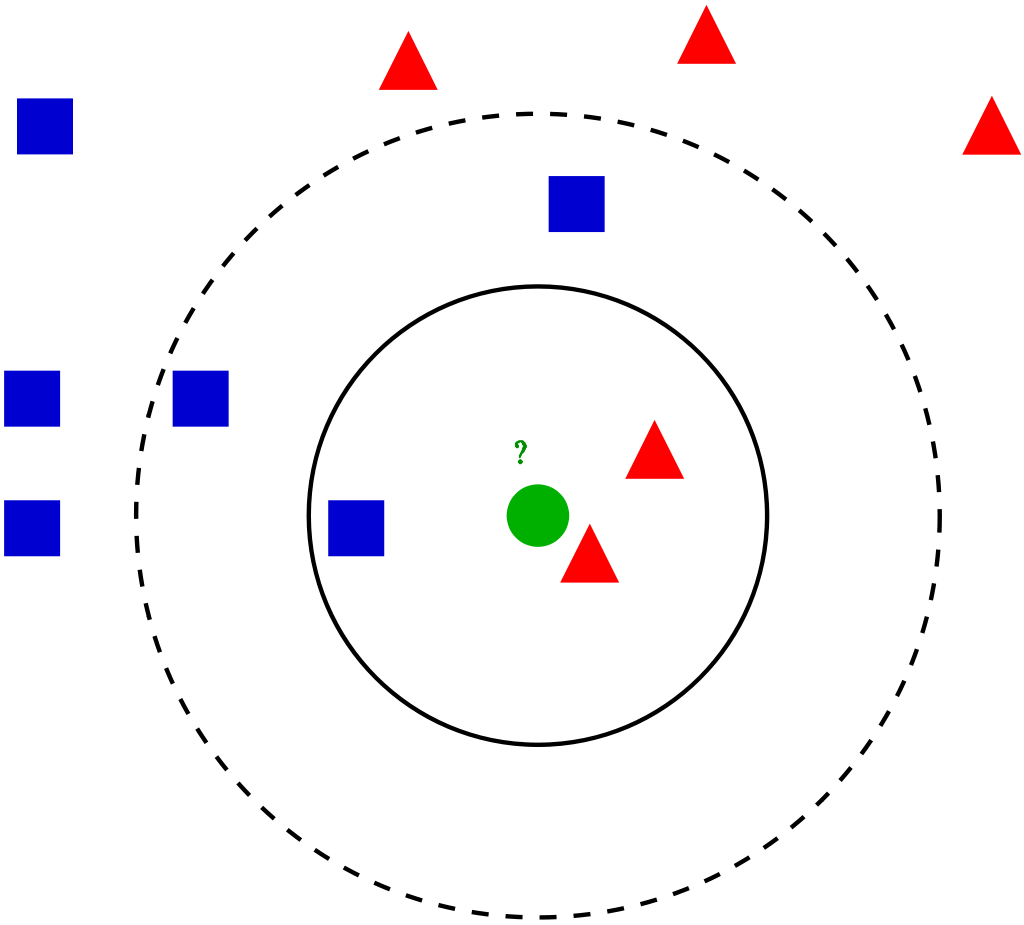
\includegraphics[width=0.5\linewidth]{knn_classification.png}
    \caption{Příklad klasifikace pomocí metody k-nejbližších sousedů.}
\end{figure}

\subsection{Gaussovský klasifikátor}

\begin{compactitem}
    \item Gaussovský klasifikátor, resp. MAP (\textit{maximum aposteriori probability}) klasifikátor.

    \begin{figure}[H]
        \centering
        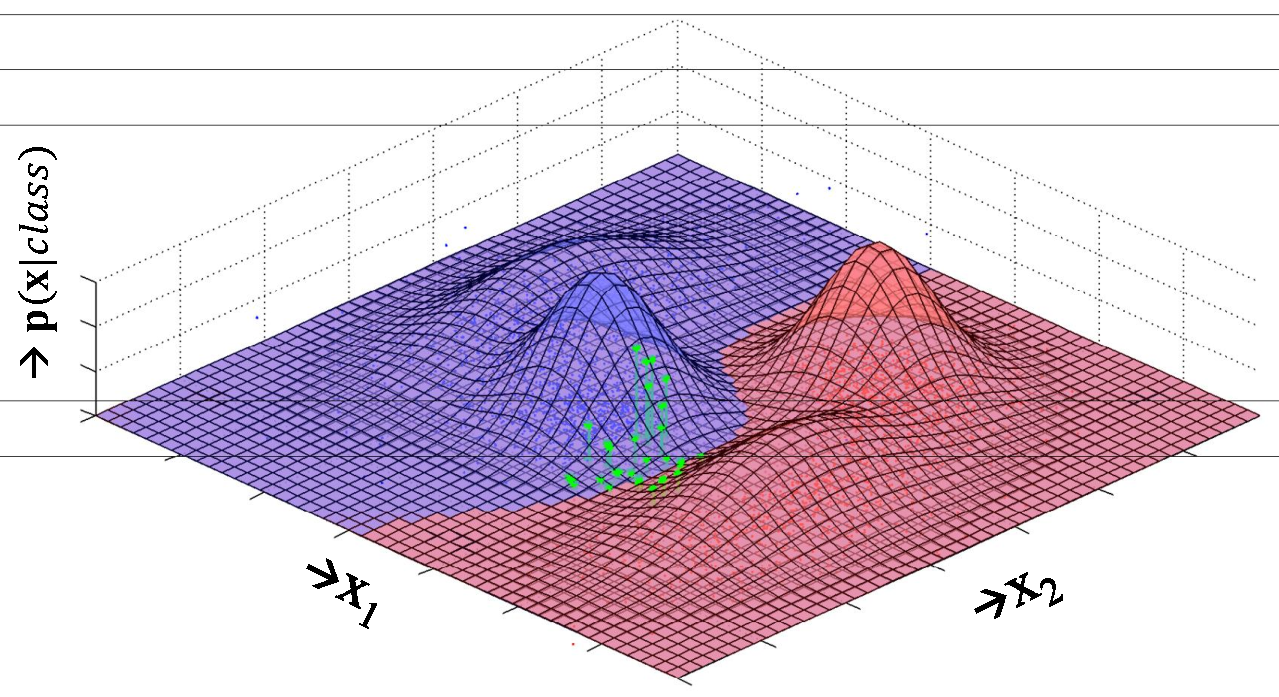
\includegraphics[width=0.9\linewidth]{gauss_classification.pdf}
        \caption{Příklad gaussovského klasifikátoru pro dvourozměrná data. Data jsou klasifikována do dvou tříd. Každá třída je modelována dvěma normálníma rozděleníma.}
    \end{figure}

    \item Při trénování modelujeme normální rozložení pravděpodobnosti v datech pro jednotlivé třídy. \begin{compactitem}
        \item Rozložení může být až n-rozměrné v závilosti na množství příznaků -- tzv. vícerozměrné gaussovo rozložení.
        \item Třída může být modelována více než jedním normálním rozložením -- tzv. multivariantní gaussovo rozložení.
    \end{compactitem}

    \item Pro klasifikaci je využívána teorie pravděpodobnosti, resp. bayesův teorém a je počítána pravděpodobnost náležitosti do určité třídy.

    \item Cílem trénování je získat pravděpodobností funkci (parametry normálních rozdělení) pro jednotlivé třídy.
    $${\displaystyle p(x) = \mathcal{N}(x, \mu, \sigma^2) = \frac{1}{\sqrt{2 \pi \sigma^2}} \cdot e^{- \frac{(x - \mu)^2}{2 \sigma^2}} }$$

    \item Při trénování provádíme tzv. odhad s maximální věrohodností (\textit{maximum likelihood estimation}) pro střední hodnotu a rozptyl. Objektivní funkce vypadá následovně:
    $$ {\displaystyle \prod_{i=1}^{n} \mathcal{N}(x_i, \mu, \sigma^2)} $$

    \item Z objektivní funkce lze odvolit, že nejlepší odhady parametrů střední hodnotu a rozptylu jsou bodové odhady:
    $$ {\displaystyle \mu = \frac{1}{n} \sum_{i=1}^n x_i } $$
    $$ {\displaystyle \sigma^2 = \frac{1}{n} \sum_{i=1}^n (x_i - \mu)^2 } $$

    \item Jak probíhá klasifikace? \begin{compactitem}
        \item Mějme dvě třídy $\omega_1$ a $\omega_2$.

        \item Pro daný datový vzorek a jeho příznak (vektor příznaků) $x$, vyber třídu $\omega_i$ s větší posteriorní pravděpodobností $P(\omega_i ~|~ x)$

        \item Vyber $\omega_1$ pokud:
        \begin{equation}
            \begin{split}
                &P(\omega_1 ~|~ x) > P (\omega_2 ~|~ x) ~\Rightarrow~ \\
                \\
                ~\Rightarrow~ &\frac{P(\omega_1) \cdot P(\omega_1 ~|~ x)}{P(x)} > \frac{P(\omega_2) \cdot P(\omega_2 ~|~ x)}{P(x)} ~\Rightarrow~ \\
                \\
                ~\Rightarrow~ &P(\omega_1 ~,~ x) > P(\omega_2 ~,~ x)
            \end{split}
        \end{equation}

    \end{compactitem}

    \item Aplikace bayesovy věty.
    \begin{figure}[H]
        \centering
        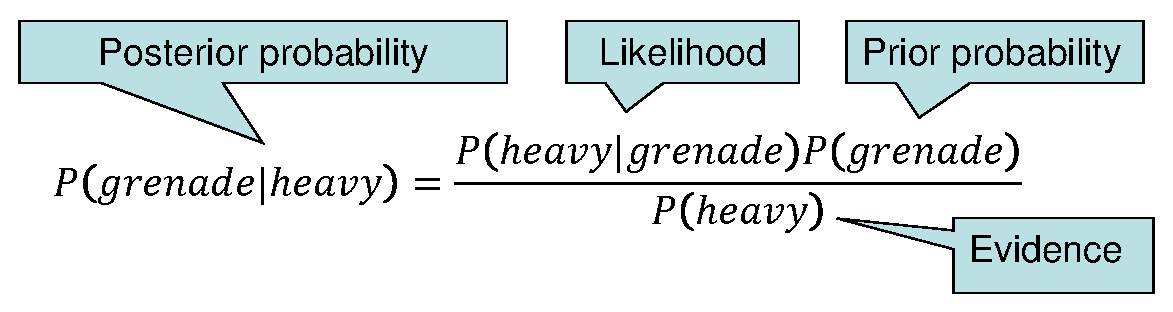
\includegraphics[width=0.75\linewidth]{bayes.pdf}
        \caption{Bayesovský teorém o podmíněné pravděpodobnosti.}
    \end{figure}

    \begin{compactitem}
        \item Apriorní pravděpodobnost (prior probability) -- Spočítáme jako marginální pravděpodobnost třídy na trénovacích datech.

        \item Věrohodnost (likelihood) -- Spočítáme jako podmíněnou pravděpodobnost.

        \item Evidence -- Spočítáme pomocí sum rule.

        \item Posterirní pravděpodobnost (posterior probability) -- Výsledek, s jakou pravděpodobností vzorek náleží jaké třídě,
    \end{compactitem}

\end{compactitem}

%%%%%%%%%%%%%%%%%%%%%%%%%%%%%%%%%%%%%%%%%%%%%%%%%%%%%%%%%%%%%%%%%%%%%%%%%%%%%%%%

\section{Diskriminativní modely klasifikátorů}

\begin{compactitem}
    \item Snažíme se z trénovacích dat neodhadovat celé funkce hustoty pravděpodobnosti, ale pouze hranice mezi třídami.

    \item Data nemusejí být Gaussovsky rozdělená (resp. každá třída odpovídat nějakému pravděpodobnostímu rozdělení).

    \item Učíme se rovnou $p(class ~|~ features)$, případně s žádnou pravděpodobností vůbec nepočítáme.

    \item Výhody/nevýhody: \begin{compactitem}
        \item Menší plýtvání parametry.
        \item Obvykle vyšší výkon s dostatečným množstvím dat.
        \item Umožňuje \uv{end-to-end} řešení.
    \end{compactitem}

    \item Modely: \begin{compactitem}
        \item Lineární logistická regrese
        \item Support Vector Machine
        \item Neuronové sítě
    \end{compactitem}
\end{compactitem}

\subsection{Lineární logistická regrese}

\todo{todo}

\subsection{Support Vector Machine}

\todo{todo}
